
\subsubsection{Prim (Baseado em Fila de Prioridade)}
O algoritmo de Prim constrói a MST incrementalmente a partir de um vértice
inicial arbitrário. A cada passo, ele escolhe a aresta de menor peso que
conecta um vértice que já está na MST a um vértice que ainda não está,
utilizando uma Fila de Prioridade (\textit{Min-Heap}). Sua complexidade de
tempo é $\mathcal{O}(E \log V)$.

\paragraph{Pseudo-Código: }\mbox{}\\
\begin{algorithm}[H]
    \SetAlgoLined
    \SetKwFunction{Prim}{Prim}
    \SetKwProg{Fn}{Função}{:}{}

    \Fn{\Prim{$adj, V$}}{
        $visitado \gets$ vetor de booleanos falso de tamanho $V$\;
        $pq \gets$ nova FilaDePrioridade() \text{guardando } $(peso, u)$\;
        $pq.push((0, 0))$ \text{ // Começa do vértice 0}\;
        $custoTotal \gets 0$\;

        \While{\text{enquanto } $pq$ \text{ não vazia}}{
            $(peso, u) \gets pq.top()$; $pq.pop()$\;
            \Se{$visitado[u]$}{
                \text{continuar}\;
            }
            $visitado[u] \gets \text{true}$\;
            $custoTotal \gets custoTotal + peso$\;

            \ParaCada{$(pesoVizinho, v) \in adj[u]$}{
                \Se{$\neg visitado[v]$}{
                    $pq.push((pesoVizinho, v))$\;
                }
            }
        }
        \Retorna $custoTotal$\;
    }
    \caption{Algoritmo de Prim}
\end{algorithm}

Veja o Prim crescendo a árvore a partir do vértice 1:\\ \vspace{0.5cm}
\noindent
\begin{minipage}[t]{0.31\textwidth}
    \centering
    \textbf{Passo 1: Início no Nó 1}\\
    \vspace{0.2cm}
    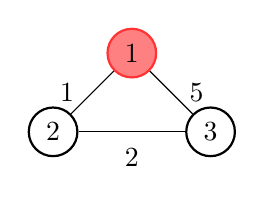
\begin{tikzpicture}[every node/.style={circle, draw, minimum size=0.5cm, thick}]
        \node[fill=red!50, draw=red!80] (1) at (0, 1) {1};
        \node (2) at (-1, 0) {2};
        \node (3) at (1, 0) {3};
        \draw (1) -- node[left, draw=none, fill=none] {1} (2);
        \draw (1) -- node[right, draw=none, fill=none] {5} (3);
        \draw (2) -- node[below, draw=none, fill=none] {2} (3);
    \end{tikzpicture}

    \vspace{0.2cm}
    \footnotesize
    \raggedright
    Inicia no vértice 1. Fila de prioridade guarda arestas incidentes: [(1, 2), (5, 3)].
\end{minipage}%
\hfill
%
\begin{minipage}[t]{0.31\textwidth}
    \centering
    \textbf{Passo 2: Expande para o Nó 2}\\
    \vspace{0.2cm}
    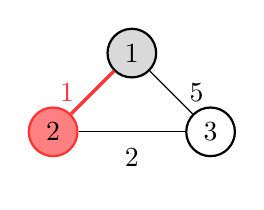
\begin{tikzpicture}[every node/.style={circle, draw, minimum size=0.5cm, thick}]
        \node[fill=gray!30] (1) at (0, 1) {1};
        \node[fill=red!50, draw=red!80] (2) at (-1, 0) {2};
        \node (3) at (1, 0) {3};
        \draw[very thick, red!80] (1) -- node[left, draw=none, fill=none] {1} (2);
        \draw (1) -- node[right, draw=none, fill=none] {5} (3);
        \draw (2) -- node[below, draw=none, fill=none] {2} (3);
    \end{tikzpicture}

    \vspace{0.2cm}
    \footnotesize
    \raggedright
    Remove menor aresta (peso 1). Visita o nó 2. Insere vizinhos de 2 na fila: [(2, 3), (5, 3)].
\end{minipage}%
\hfill
%
\begin{minipage}[t]{0.31\textwidth}
    \centering
    \textbf{Passo 3: Expande para o Nó 3}\\
    \vspace{0.2cm}
    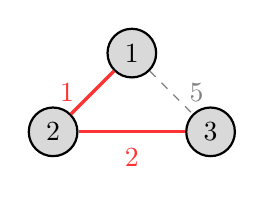
\begin{tikzpicture}[every node/.style={circle, draw, minimum size=0.5cm, thick}]
        \node[fill=gray!30] (1) at (0, 1) {1};
        \node[fill=gray!30] (2) at (-1, 0) {2};
        \node[fill=gray!30] (3) at (1, 0) {3};
        \draw[very thick, red!80] (1) -- node[left, draw=none, fill=none] {1} (2);
        \draw[dashed, gray] (1) -- node[right, draw=none, fill=none] {5} (3);
        \draw[very thick, red!80] (2) -- node[below, draw=none, fill=none] {2} (3);
    \end{tikzpicture}

    \vspace{0.2cm}
    \footnotesize
    \raggedright
    Remove menor aresta (peso 2). Visita o nó 3. Todos conectados! Custo total: 3.
\end{minipage}

\vspace{0.3cm}

\paragraph{Implementação: }\mbox{}\\
\textbf{Python: }
\begin{lstlisting}[language=Python]
import heapq

def prim(n, adj):
    # adj[u] = lista de tuplas (peso, v)
    visitado = [False] * n
    pq = [(0, 0)] # (peso, vertice)
    custo_total = 0
    
    while pq:
        peso, u = heapq.heappop(pq)
        
        if visitado[u]:
            continue
            
        visitado[u] = True
        custo_total += peso
        
        for peso_vizinho, v in adj[u]:
            if not visitado[v]:
                heapq.heappush(pq, (peso_vizinho, v))
                
    return custo_total
\end{lstlisting}

\vspace{0.3cm}
\textbf{C++:}
\begin{lstlisting}[language=C++]
int prim(int n, const vector<vector<pair<int, int>>>& adj) {
    vector<bool> visitado(n, false);
    priority_queue<pair<int, int>, vector<pair<int, int>>, greater<pair<int, int>>> pq;
    
    pq.push({0, 0}); // {peso, vertice}
    int custoTotal = 0;
    
    while (!pq.empty()) {
        int peso = pq.top().first;
        int u = pq.top().second;
        pq.pop();
        
        if (visitado[u]) continue;
        visitado[u] = true;
        custoTotal += peso;
        
        for (auto& edge : adj[u]) {
            int pesoVizinho = edge.first;
            int v = edge.second;
            
            if (!visitado[v]) {
                pq.push({pesoVizinho, v});
            }
        }
    }
    return custoTotal;
}
\end{lstlisting}
\newpage